\documentclass{article}
\usepackage{/Users/miles/Documents/latex/hw}

%% Extra packages
\usepackage{mathtools}  % Starred matrix environments
\usepackage{tikz}   % Rotation diagram

%% Metadata
\renewcommand{\Title}{Rotation Matrix Assignment}
\renewcommand{\Course}{PHYS 350}
\renewcommand{\Date}{November 4, 2016}
\renewcommand{\Author}{Miles Moser}

\begin{document}
\insertTitle

\textbf{Problem.} Consider a vector $\vb{r}$ that lies in a Cartesian coordinate system. Now imagine a second Cartesian coordinate system, in the same plane as the first and sharing the same origin, but whose axes are rotated counterclockwise by an angle $\theta$:

\begin{center}
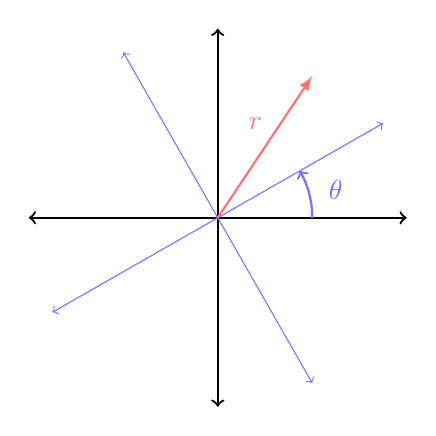
\begin{tikzpicture}[scale = 0.6]
  \draw [<->, thick](-4,0) -- (4,0); %x-axis
  \draw [<->, thick](0,-4) -- (0,4); %y-axis
  \draw [color={blue!55}, <->](-3.5,-2) -- (3.5,2); %x'-axis
  \draw [color={blue!55}, <->](2,-3.5) -- (-2,3.5); %y'-axis
  \draw [-latex, color={red!55}, thick](0,0) -- (2,3); %vector
  \draw [->,color={blue!55}, thick](2,0) arc (0:30:2); %angle marker
  
  \node[color={blue!55}] at (2.5,0.6) {$\theta$};
  \node[color={red!55}] at (0.8,2) {$\vb{r}$};
\end{tikzpicture}
\end{center}

Now, if we want to express $\vb{r}$ as a new vector $\vb{r'}$ relative to a new coordinate system, we can multiply it by a transformation matrix $\mathbf{A}$ such that $\vb{r'} = \mathbf{A}\vb{r}$. For a two-dimensional rotation like the above, it turns out the transformation matrix is given by the following:
\[
    \mathbf{A} =
    \begin{pmatrix*}[r]
    \cos\theta & \sin\theta \\
    -\sin\theta & \cos\theta
    \end{pmatrix*}
\]

Intuitively, it follows that performing multiple rotations with multiple matrices could always be expressed as a single, composite transformation. In particular, performing the same rotational transformation through angle $\theta$ twice should yield the same result as performing a single rotation through angle $2\theta$. We can show this mathematically through matrix manipulation.

\textbf{Solution.} If we rotate $\vb{r}$ by angle $\theta$, we'll have $\vb{r'} = \mathbf{A}\vb{r}$. If we perform the same transformation again, we'll have:
\[
    \vb{r''} = \mathbf{A}\vb{r'} = \mathbf{A}(\mathbf{A}\vb{r}\,) = \mathbf{A}^2 \vb{r}
\]

On the other hand, if we had simply rotated $\vb{r}$ by $2\theta$ to begin with, we would have:
\[
    \vb{r''} = \mathbf{B}\vb{r}\text{, where }\mathbf{B} =
    \begin{pmatrix*}[r]
    \cos2\theta & \sin2\theta \\
    -\sin2\theta & \cos2\theta
    \end{pmatrix*}
\]

So, to show that these transformations are the same, we just have to show that $\mathbf{A}^2 = \mathbf{B}$:
\[
    \begin{aligned}
    \mathbf{A}^2 &= 
    \begin{pmatrix*}[r]
    \cos\theta & \sin\theta \\
    -\sin\theta & \cos\theta
    \end{pmatrix*}
    \begin{pmatrix*}[r]
    \cos\theta & \sin\theta \\
    -\sin\theta & \cos\theta
    \end{pmatrix*} \\
    &= \begin{pmatrix*}[c]
    \cos^2\theta - \sin^2\theta & \cos\theta\sin\theta + \sin\theta\cos\theta\\
    -\sin\theta\cos\theta - \cos\theta\sin\theta & -\sin^2\theta + \cos^2\theta
    \end{pmatrix*} \\
    &= \begin{pmatrix*}[c]
    \cos^2\theta - \sin^2\theta & 2\sin\theta\cos\theta\\
    -2\sin\theta\cos\theta & \cos^2\theta - \sin^2\theta
    \end{pmatrix*}
    \end{aligned}
\]

We can use the following double-angle trigonometric identities:
\[
    \begin{aligned}
    \sin2\theta &= 2\sin\theta\cos\theta \\
    \cos2\theta &= \cos^2 \theta - \sin^2 \theta
    \end{aligned}
\]

Substituting:
\[
    \mathbf{A}^2 =
    \begin{pmatrix*}[r]
    \cos2\theta & \sin2\theta \\
    -\sin2\theta & \cos2\theta
    \end{pmatrix*}
    = \mathbf{B}, \>\>\text{as required.}
\]

\end{document}